\documentclass[11pt,a4paper]{article}
\usepackage[margin=22mm]{geometry}
\usepackage[T1]{fontenc}
\usepackage{lmodern}
\usepackage{amsmath,booktabs,graphicx}
\graphicspath{{figures/}}
\setlength{\parindent}{0pt}
\setlength{\parskip}{5pt}
\setlength{\topsep}{4pt}
\setlength{\partopsep}{0pt}
\setlength{\smallskipamount}{4pt plus 1pt minus 1pt}
\setlength{\medskipamount}{10pt plus 2pt minus 1pt}
\setlength{\bigskipamount}{14pt plus 3pt minus 2pt}
\setlength{\tabcolsep}{6pt}
\renewcommand{\arraystretch}{1.12}
\newcommand{\sectiongap}{\par\vspace{9mm}}
\newcommand{\confusion}[3]{%
  \begin{minipage}[t]{0.24\linewidth}
  \setlength{\parskip}{0pt}\centering
  \textbf{#1}\par\vspace{4pt}
  {\normalsize\setlength{\tabcolsep}{2.5pt}%
  \renewcommand{\arraystretch}{1.02}%
  \begin{tabular}{r@{\quad}#2}\toprule
  #3
  \bottomrule\end{tabular}}
  \end{minipage}}
\begin{document}
\begin{titlepage}



\centering
\vspace*{2cm}
{\Large\textbf{ASSIGNMENT REPORT-8}}\\[0.7cm]
{\large\textbf{CLASSIFIERS WITH AND WITHOUT PCA}}\\[1.7cm]
\textbf{Submitted by:}\\[0.4cm]
\textbf{KARTHIKEYAN M} [26120004]\\[0.3cm]
\textbf{MIRTHULA M} [26120121]\\[1.8cm]
\textbf{Under the guidance of:}\\[0.4cm]
\textbf{HEMA ARUNACHALAM MURTHY}\\[1.5cm]
\textbf{For the subject}\\[0.4cm]
{\Large\textbf{Pattern Recognition and Machine Learning}}\\[0.3cm]
\textbf{(26AI5707)}
\vspace{2cm}

{\textbf{DEPARTMENT OF COMPUTER SCIENCE \& ENGINEERING}\\[0.3cm]
\textbf{SHIV NADAR UNIVERSITY, CHENNAI}\\[0.3cm]
\textbf{NOVEMBER 2026}}
\end{titlepage}
\section*{Introduction}

This assignment is all about comparing different classifiers such as GMM, KNN, LDA, SVM and also considering the reduced dimensions versions (i.e.) before and after PCA across four datasets for all 4 classifiers. For each dataset we first observe a 2D PCA version and then start building the models and record their confusion matrices and their accuracy.

\par\medskip
\noindent\begin{minipage}{\linewidth}
{\Large\textbf{1. Synthetic data}}\par\medskip
\begin{center}\small
\begin{tabular}{lrrrrrr}\toprule
Labels & Classes & Train & Validation & Test & Features $d$ & PCA $k$ \\ \midrule
$\{0,1\}$ & 2 & 12000 & 4000 & 4000 & 16 & 8 \\ \bottomrule
\end{tabular}\end{center}
\vspace{3mm}
\begin{center}
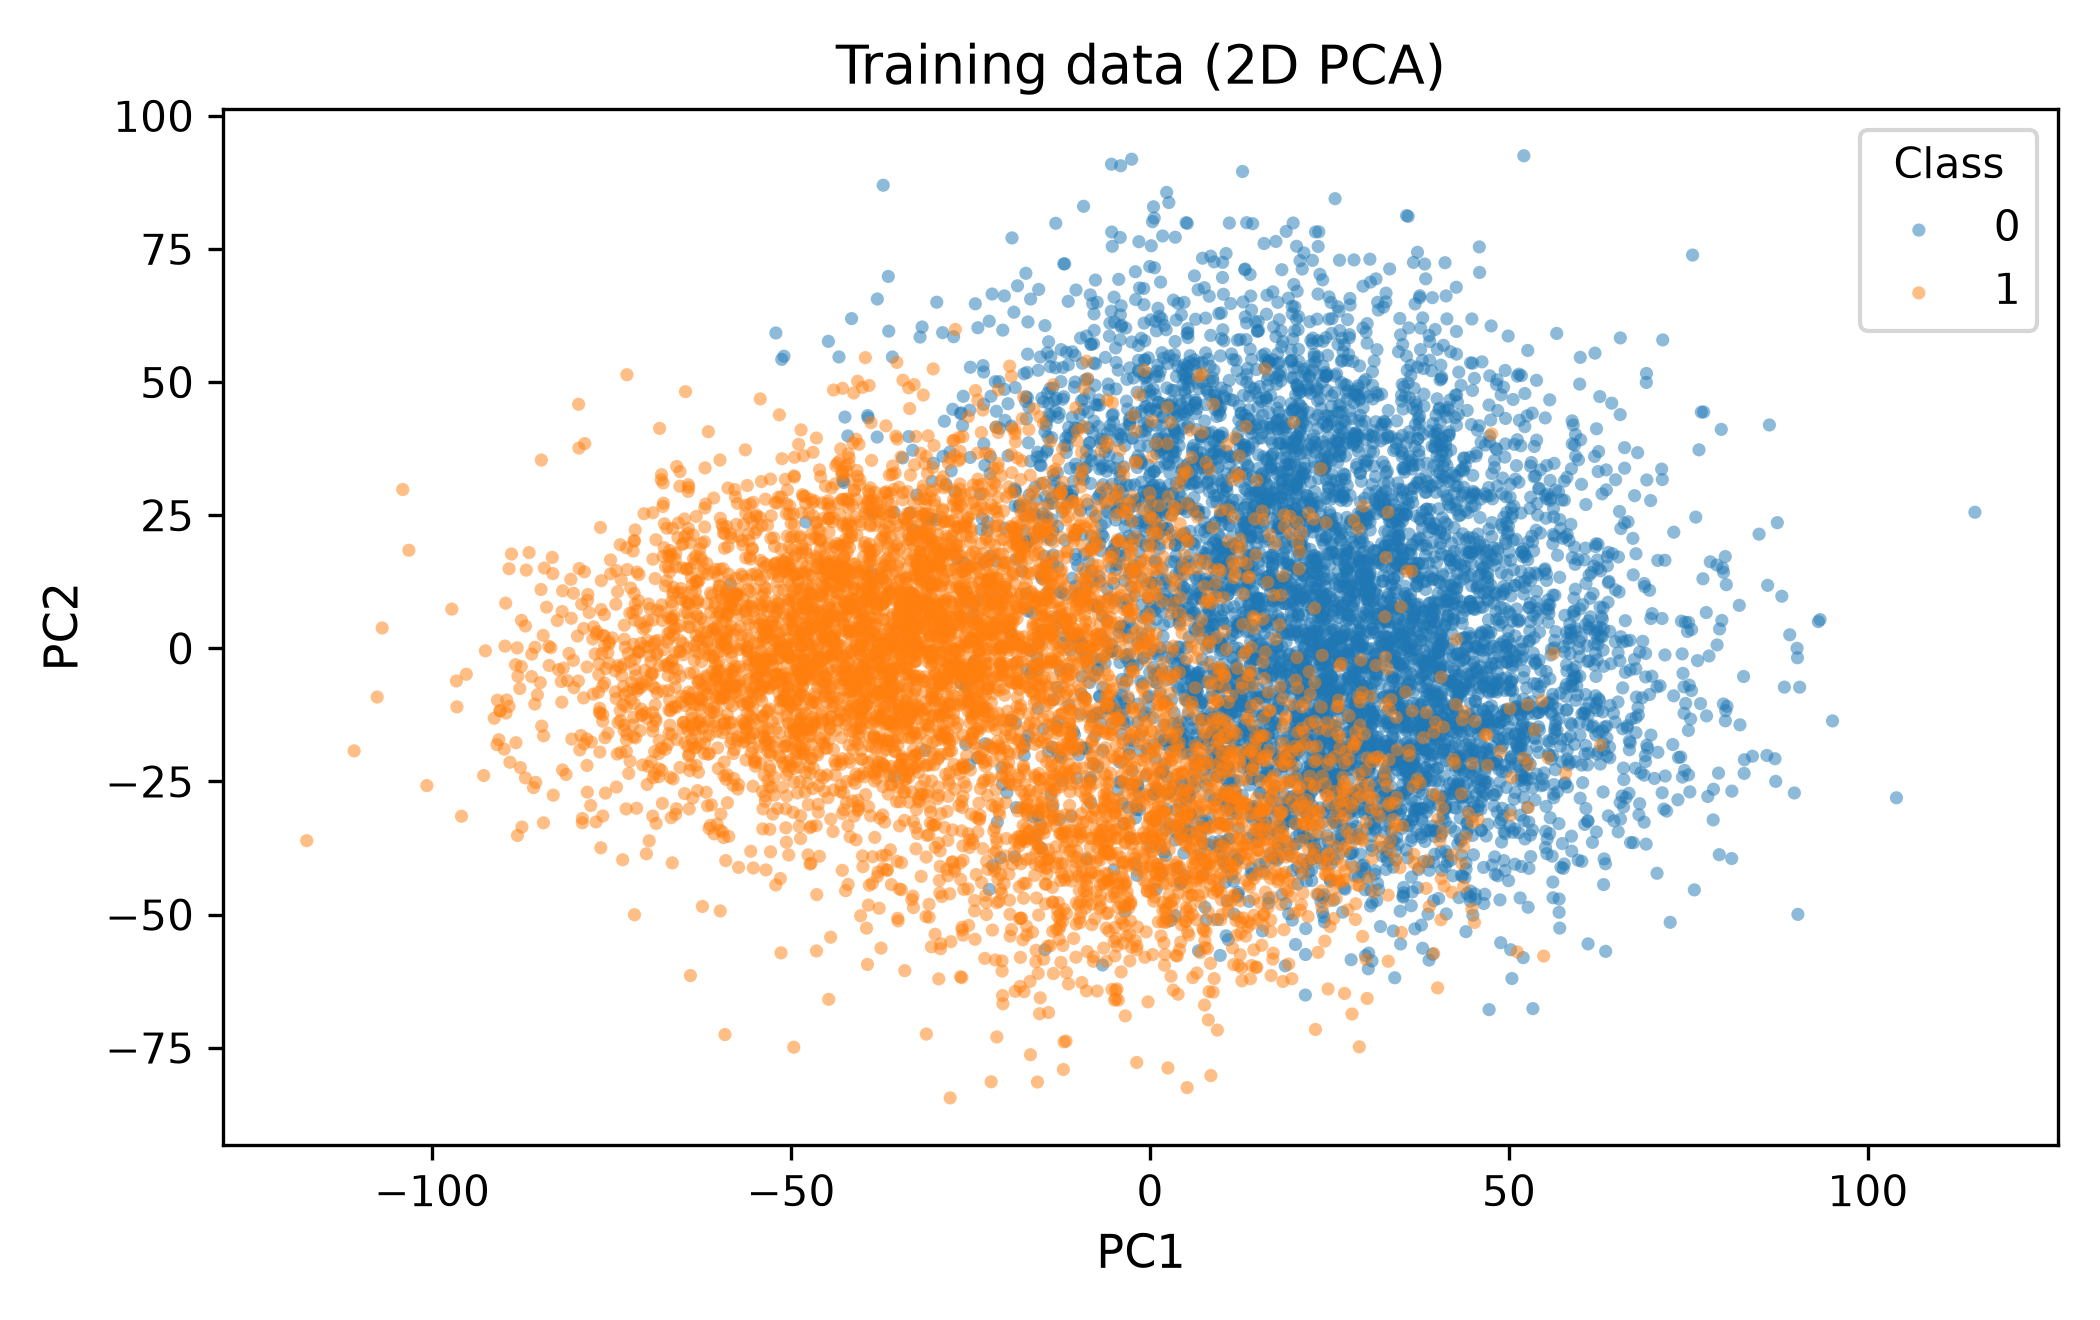
\includegraphics[width=0.90\linewidth]{synthetic_data_pca.png}
\end{center}\end{minipage}\sectiongap
\noindent\begin{minipage}{\linewidth}
\textbf{Accuracy (\%)}\par
\begin{center}\small
\setlength{\tabcolsep}{9pt}
\renewcommand{\arraystretch}{1.15}
\begin{tabular}{lrrrr}\toprule
 & \multicolumn{2}{c}{Without PCA} & \multicolumn{2}{c}{With PCA} \\
\cmidrule(lr){2-3}\cmidrule(lr){4-5}
Classifier & Validation & Test & Validation & Test \\ \midrule
GMM & 100.00 & \textbf{100.00} & 98.40 & \textbf{98.33} \\
KNN & 99.48 & 99.58 & 97.30 & 97.85 \\
LDA & 94.50 & 94.78 & 91.08 & 90.75 \\
SVM & 99.68 & 99.75 & 96.38 & 96.40 \\
\bottomrule\end{tabular}\end{center}
\end{minipage}\par\clearpage
\noindent\begin{minipage}{\linewidth}
\begin{center}
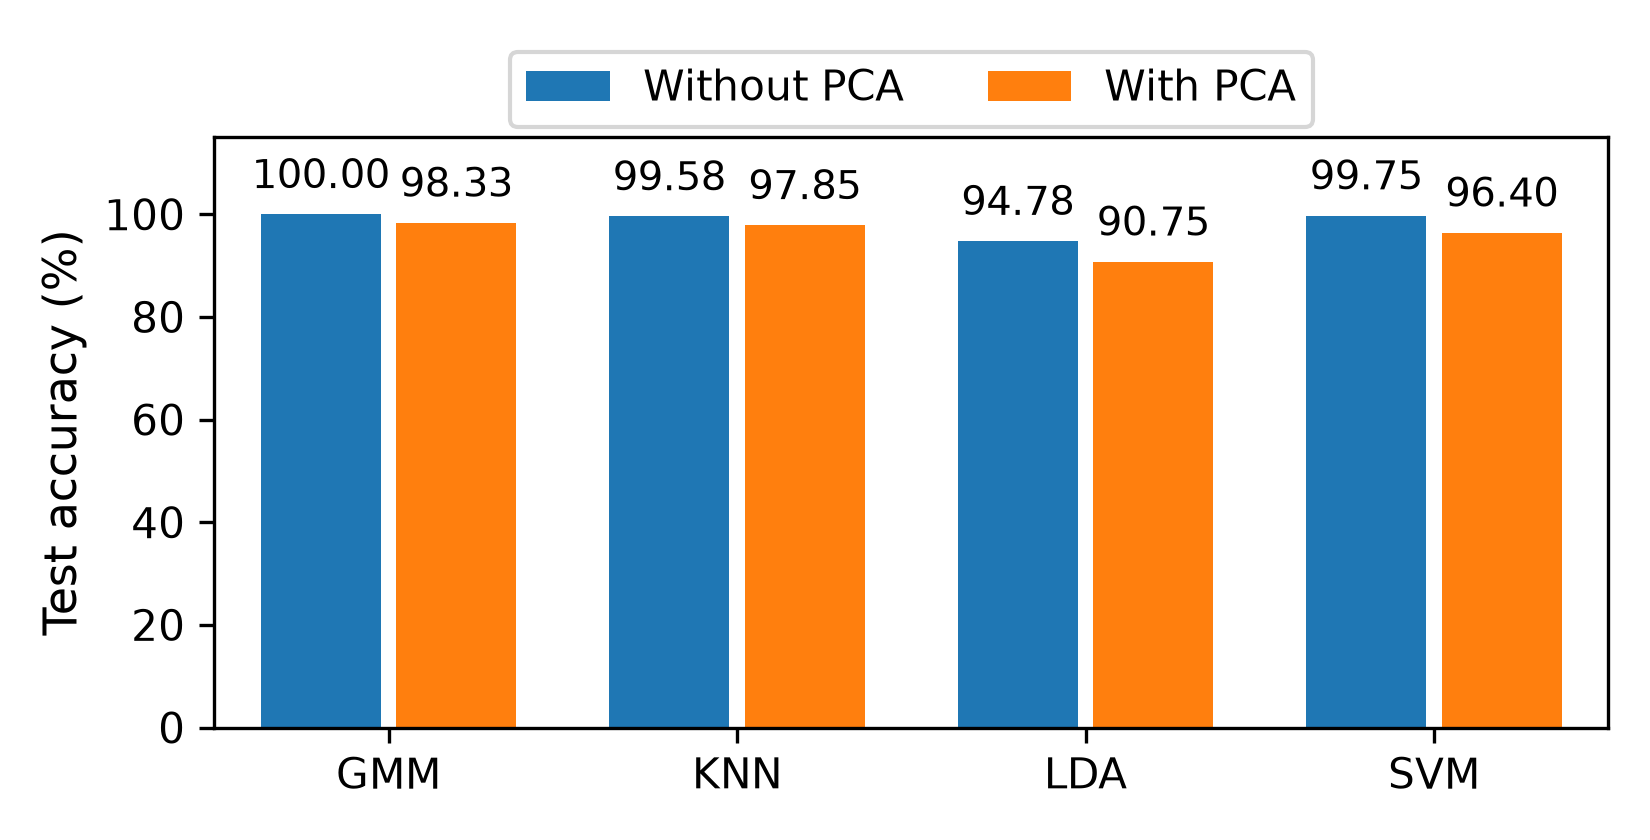
\includegraphics[width=0.70\linewidth]{synthetic_data_accuracy.png}
\end{center}\end{minipage}\sectiongap
\noindent\begin{minipage}{\linewidth}
\textbf{Test confusion matrices}\hfill{\footnotesize Rows: actual; columns: predicted.}\par\smallskip
\textbf{Without PCA}\par\smallskip
\confusion{GMM}{rr}{
 & \textbf{0} & \textbf{1} \\ \midrule
\textbf{0} & 2001 & 0 \\
\textbf{1} & 0 & 1999 \\
}\hfill
\confusion{KNN}{rr}{
 & \textbf{0} & \textbf{1} \\ \midrule
\textbf{0} & 1985 & 16 \\
\textbf{1} & 1 & 1998 \\
}\hfill
\confusion{LDA}{rr}{
 & \textbf{0} & \textbf{1} \\ \midrule
\textbf{0} & 1880 & 121 \\
\textbf{1} & 88 & 1911 \\
}\hfill
\confusion{SVM}{rr}{
 & \textbf{0} & \textbf{1} \\ \midrule
\textbf{0} & 1995 & 6 \\
\textbf{1} & 4 & 1995 \\
}
\par\medskip
\textbf{With PCA}\par\smallskip
\confusion{GMM}{rr}{
 & \textbf{0} & \textbf{1} \\ \midrule
\textbf{0} & 1962 & 39 \\
\textbf{1} & 28 & 1971 \\
}\hfill
\confusion{KNN}{rr}{
 & \textbf{0} & \textbf{1} \\ \midrule
\textbf{0} & 1947 & 54 \\
\textbf{1} & 32 & 1967 \\
}\hfill
\confusion{LDA}{rr}{
 & \textbf{0} & \textbf{1} \\ \midrule
\textbf{0} & 1839 & 162 \\
\textbf{1} & 208 & 1791 \\
}\hfill
\confusion{SVM}{rr}{
 & \textbf{0} & \textbf{1} \\ \midrule
\textbf{0} & 1931 & 70 \\
\textbf{1} & 74 & 1925 \\
}
\sectiongap
\textbf{Observations}\par

Eventhough there is an overlap in the 2D projection, GMM still gets 100\% validation and test accuracy using when we use all the 16 features. This demonstrates the capability of GMMs as it can also create non-linear boundaries as well. PCA to eight features reduces the test accuracy to 98.33\%.

\end{minipage}\par\bigskip
\clearpage
\noindent\begin{minipage}{\linewidth}
{\Large\textbf{2. Image features}}\par\medskip
\begin{center}\small
\begin{tabular}{lrrrrrr}\toprule
Labels & Classes & Train & Validation & Test & Features $d$ & PCA $k$ \\ \midrule
$\{0,1,2,3,4\}$ & 5 & 2000 & 500 & 500 & 36 & 18 \\ \bottomrule
\end{tabular}\end{center}
\vspace{3mm}
\begin{center}
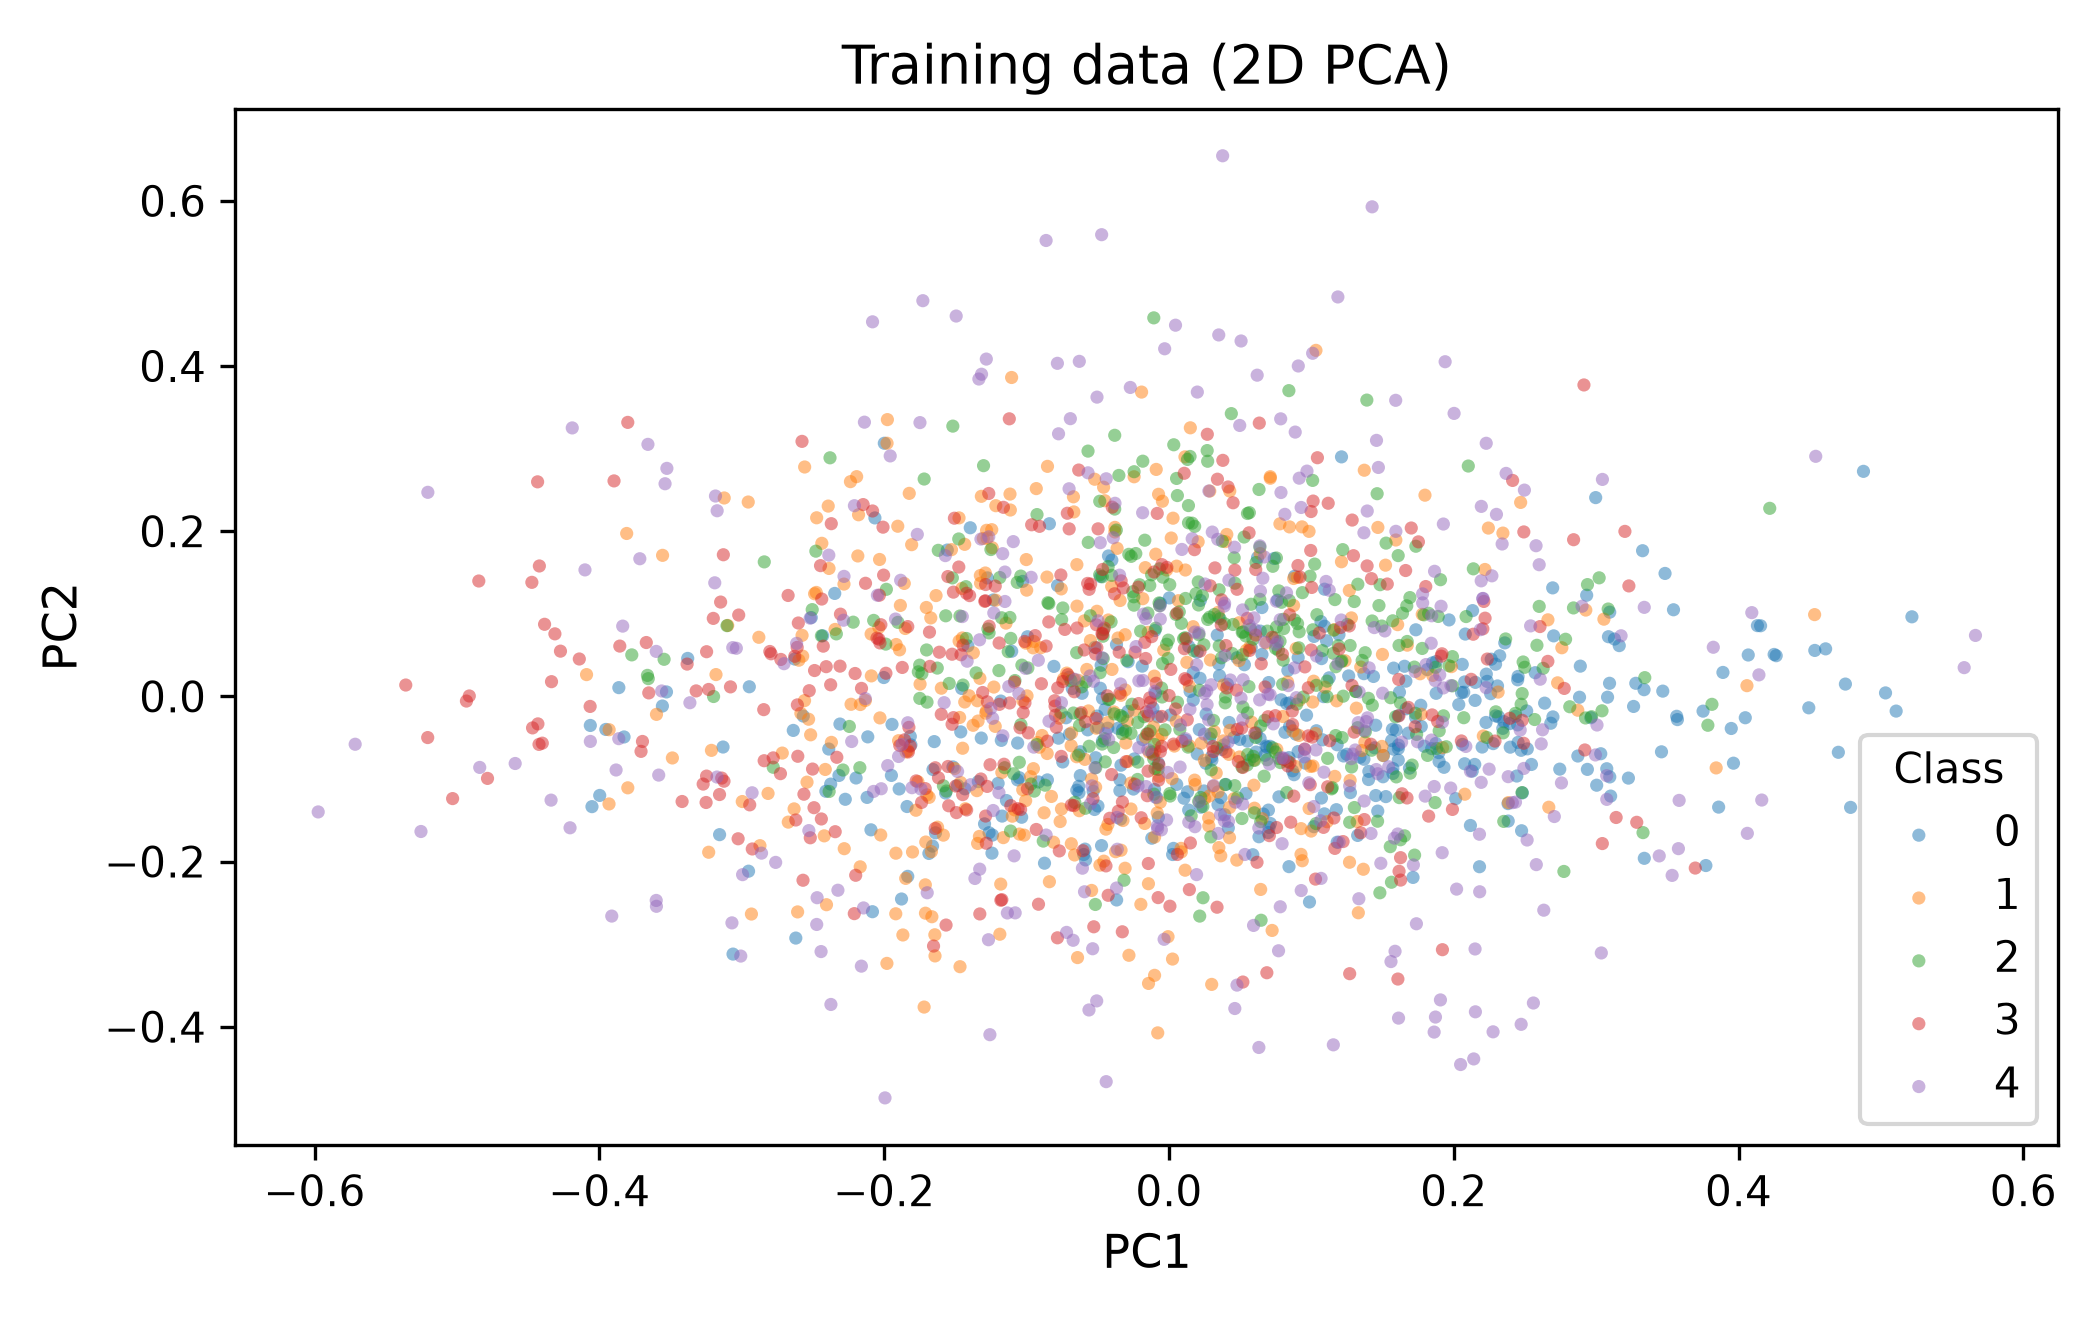
\includegraphics[width=0.90\linewidth]{image_features_pca.png}
\end{center}\end{minipage}\sectiongap
\noindent\begin{minipage}{\linewidth}
\textbf{Accuracy (\%)}\par
\begin{center}\small
\setlength{\tabcolsep}{9pt}
\renewcommand{\arraystretch}{1.15}
\begin{tabular}{lrrrr}\toprule
 & \multicolumn{2}{c}{Without PCA} & \multicolumn{2}{c}{With PCA} \\
\cmidrule(lr){2-3}\cmidrule(lr){4-5}
Classifier & Validation & Test & Validation & Test \\ \midrule
GMM & 62.60 & 57.40 & 63.40 & \textbf{58.80} \\
KNN & 55.60 & 51.40 & 59.00 & 52.20 \\
LDA & 58.80 & 57.60 & 59.60 & 56.20 \\
SVM & 63.00 & \textbf{62.20} & 64.20 & 57.60 \\
\bottomrule\end{tabular}\end{center}
\end{minipage}\par\clearpage
\noindent\begin{minipage}{\linewidth}
\begin{center}
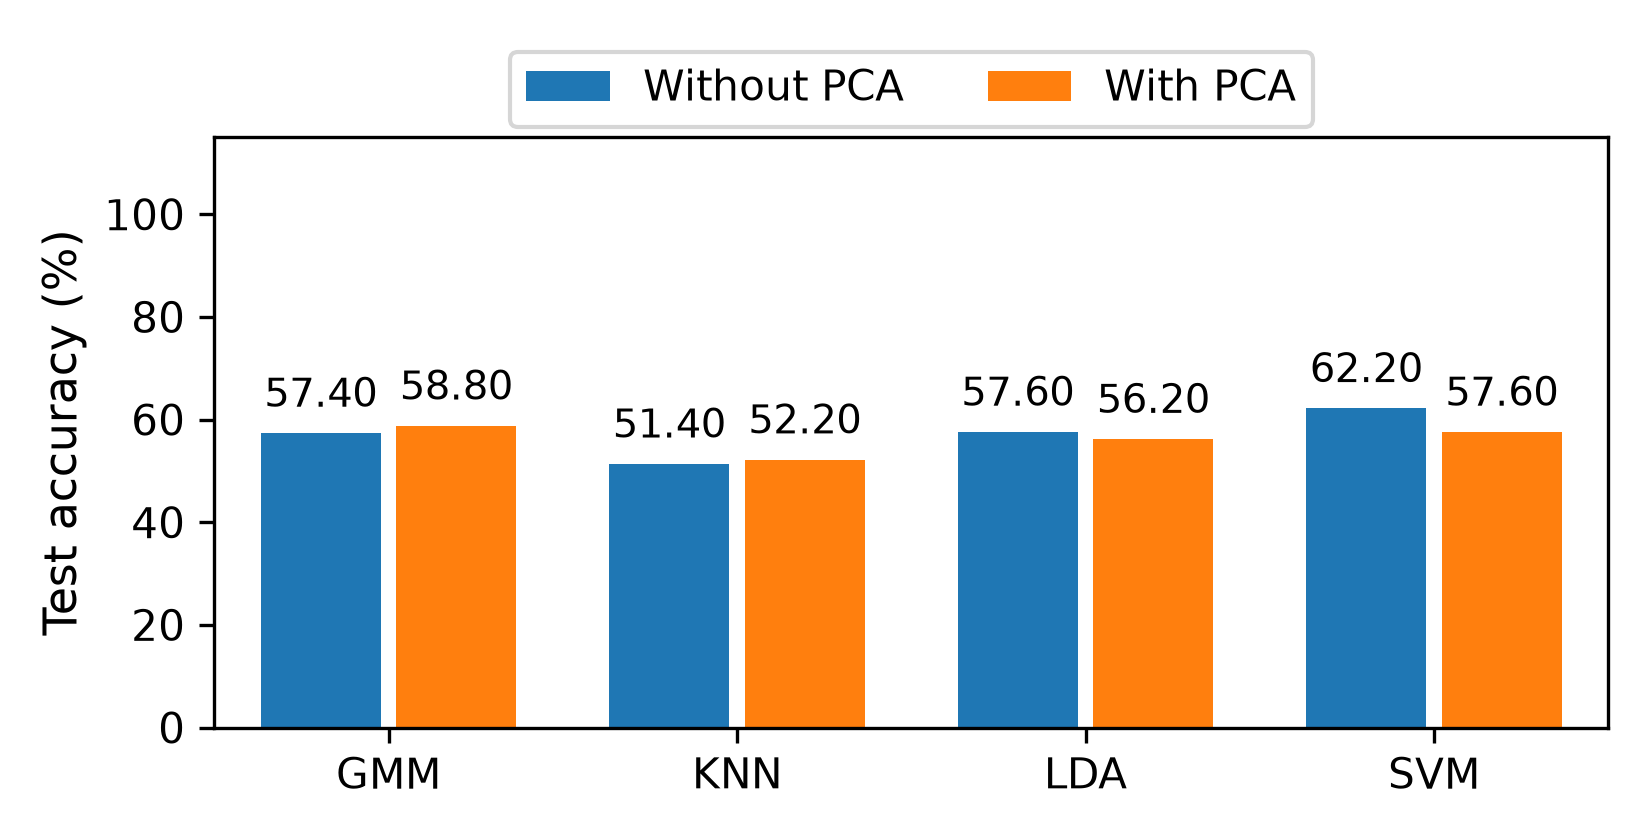
\includegraphics[width=0.70\linewidth]{image_features_accuracy.png}
\end{center}\end{minipage}\sectiongap
\noindent\begin{minipage}{\linewidth}
\textbf{Test confusion matrices}\hfill{\footnotesize Rows: actual; columns: predicted.}\par\smallskip
\textbf{Without PCA}\par\smallskip
\confusion{GMM}{rrrrr}{
 & \textbf{0} & \textbf{1} & \textbf{2} & \textbf{3} & \textbf{4} \\ \midrule
\textbf{0} & 62 & 7 & 16 & 9 & 6 \\
\textbf{1} & 7 & 75 & 8 & 5 & 5 \\
\textbf{2} & 6 & 3 & 68 & 15 & 8 \\
\textbf{3} & 8 & 4 & 29 & 37 & 22 \\
\textbf{4} & 4 & 3 & 18 & 30 & 45 \\
}\hfill
\confusion{KNN}{rrrrr}{
 & \textbf{0} & \textbf{1} & \textbf{2} & \textbf{3} & \textbf{4} \\ \midrule
\textbf{0} & 61 & 10 & 18 & 5 & 6 \\
\textbf{1} & 6 & 73 & 14 & 5 & 2 \\
\textbf{2} & 8 & 5 & 67 & 14 & 6 \\
\textbf{3} & 11 & 6 & 47 & 26 & 10 \\
\textbf{4} & 11 & 6 & 30 & 23 & 30 \\
}\hfill
\confusion{LDA}{rrrrr}{
 & \textbf{0} & \textbf{1} & \textbf{2} & \textbf{3} & \textbf{4} \\ \midrule
\textbf{0} & 66 & 13 & 12 & 6 & 3 \\
\textbf{1} & 7 & 75 & 9 & 6 & 3 \\
\textbf{2} & 8 & 6 & 64 & 20 & 2 \\
\textbf{3} & 13 & 10 & 31 & 32 & 14 \\
\textbf{4} & 7 & 7 & 16 & 19 & 51 \\
}\hfill
\confusion{SVM}{rrrrr}{
 & \textbf{0} & \textbf{1} & \textbf{2} & \textbf{3} & \textbf{4} \\ \midrule
\textbf{0} & 68 & 10 & 7 & 8 & 7 \\
\textbf{1} & 6 & 81 & 8 & 3 & 2 \\
\textbf{2} & 7 & 6 & 61 & 13 & 13 \\
\textbf{3} & 11 & 7 & 22 & 34 & 26 \\
\textbf{4} & 5 & 2 & 14 & 12 & 67 \\
}
\par\medskip
\textbf{With PCA}\par\smallskip
\confusion{GMM}{rrrrr}{
 & \textbf{0} & \textbf{1} & \textbf{2} & \textbf{3} & \textbf{4} \\ \midrule
\textbf{0} & 62 & 14 & 10 & 10 & 4 \\
\textbf{1} & 5 & 77 & 6 & 7 & 5 \\
\textbf{2} & 5 & 4 & 72 & 13 & 6 \\
\textbf{3} & 11 & 5 & 35 & 33 & 16 \\
\textbf{4} & 7 & 3 & 14 & 26 & 50 \\
}\hfill
\confusion{KNN}{rrrrr}{
 & \textbf{0} & \textbf{1} & \textbf{2} & \textbf{3} & \textbf{4} \\ \midrule
\textbf{0} & 63 & 12 & 15 & 7 & 3 \\
\textbf{1} & 6 & 80 & 10 & 2 & 2 \\
\textbf{2} & 10 & 5 & 64 & 13 & 8 \\
\textbf{3} & 18 & 5 & 43 & 24 & 10 \\
\textbf{4} & 17 & 7 & 26 & 20 & 30 \\
}\hfill
\confusion{LDA}{rrrrr}{
 & \textbf{0} & \textbf{1} & \textbf{2} & \textbf{3} & \textbf{4} \\ \midrule
\textbf{0} & 66 & 11 & 11 & 7 & 5 \\
\textbf{1} & 7 & 75 & 8 & 7 & 3 \\
\textbf{2} & 7 & 6 & 65 & 19 & 3 \\
\textbf{3} & 14 & 8 & 34 & 26 & 18 \\
\textbf{4} & 7 & 10 & 17 & 17 & 49 \\
}\hfill
\confusion{SVM}{rrrrr}{
 & \textbf{0} & \textbf{1} & \textbf{2} & \textbf{3} & \textbf{4} \\ \midrule
\textbf{0} & 63 & 13 & 8 & 11 & 5 \\
\textbf{1} & 6 & 76 & 6 & 9 & 3 \\
\textbf{2} & 9 & 6 & 53 & 18 & 14 \\
\textbf{3} & 8 & 8 & 30 & 31 & 23 \\
\textbf{4} & 7 & 3 & 12 & 13 & 65 \\
}
\sectiongap
\textbf{Observations}\par
Here we see PCA slightly improves GMM and KNN test accuracy, but on the other hand reduces the same for LDA and SVM. SVM performed best without PCA; GMM performed best along with PCA.

\end{minipage}\par\bigskip
\clearpage
\noindent\begin{minipage}{\linewidth}
{\Large\textbf{3. MNIST}}\par\medskip
\begin{center}\small
\begin{tabular}{lrrrrrr}\toprule
Labels & Classes & Train & Validation & Test & Features $d$ & PCA $k$ \\ \midrule
$\{2,3,9\}$ & 3 & 14424 & 3614 & 3051 & 784 & 50 \\ \bottomrule
\end{tabular}\end{center}
\vspace{3mm}
\begin{center}
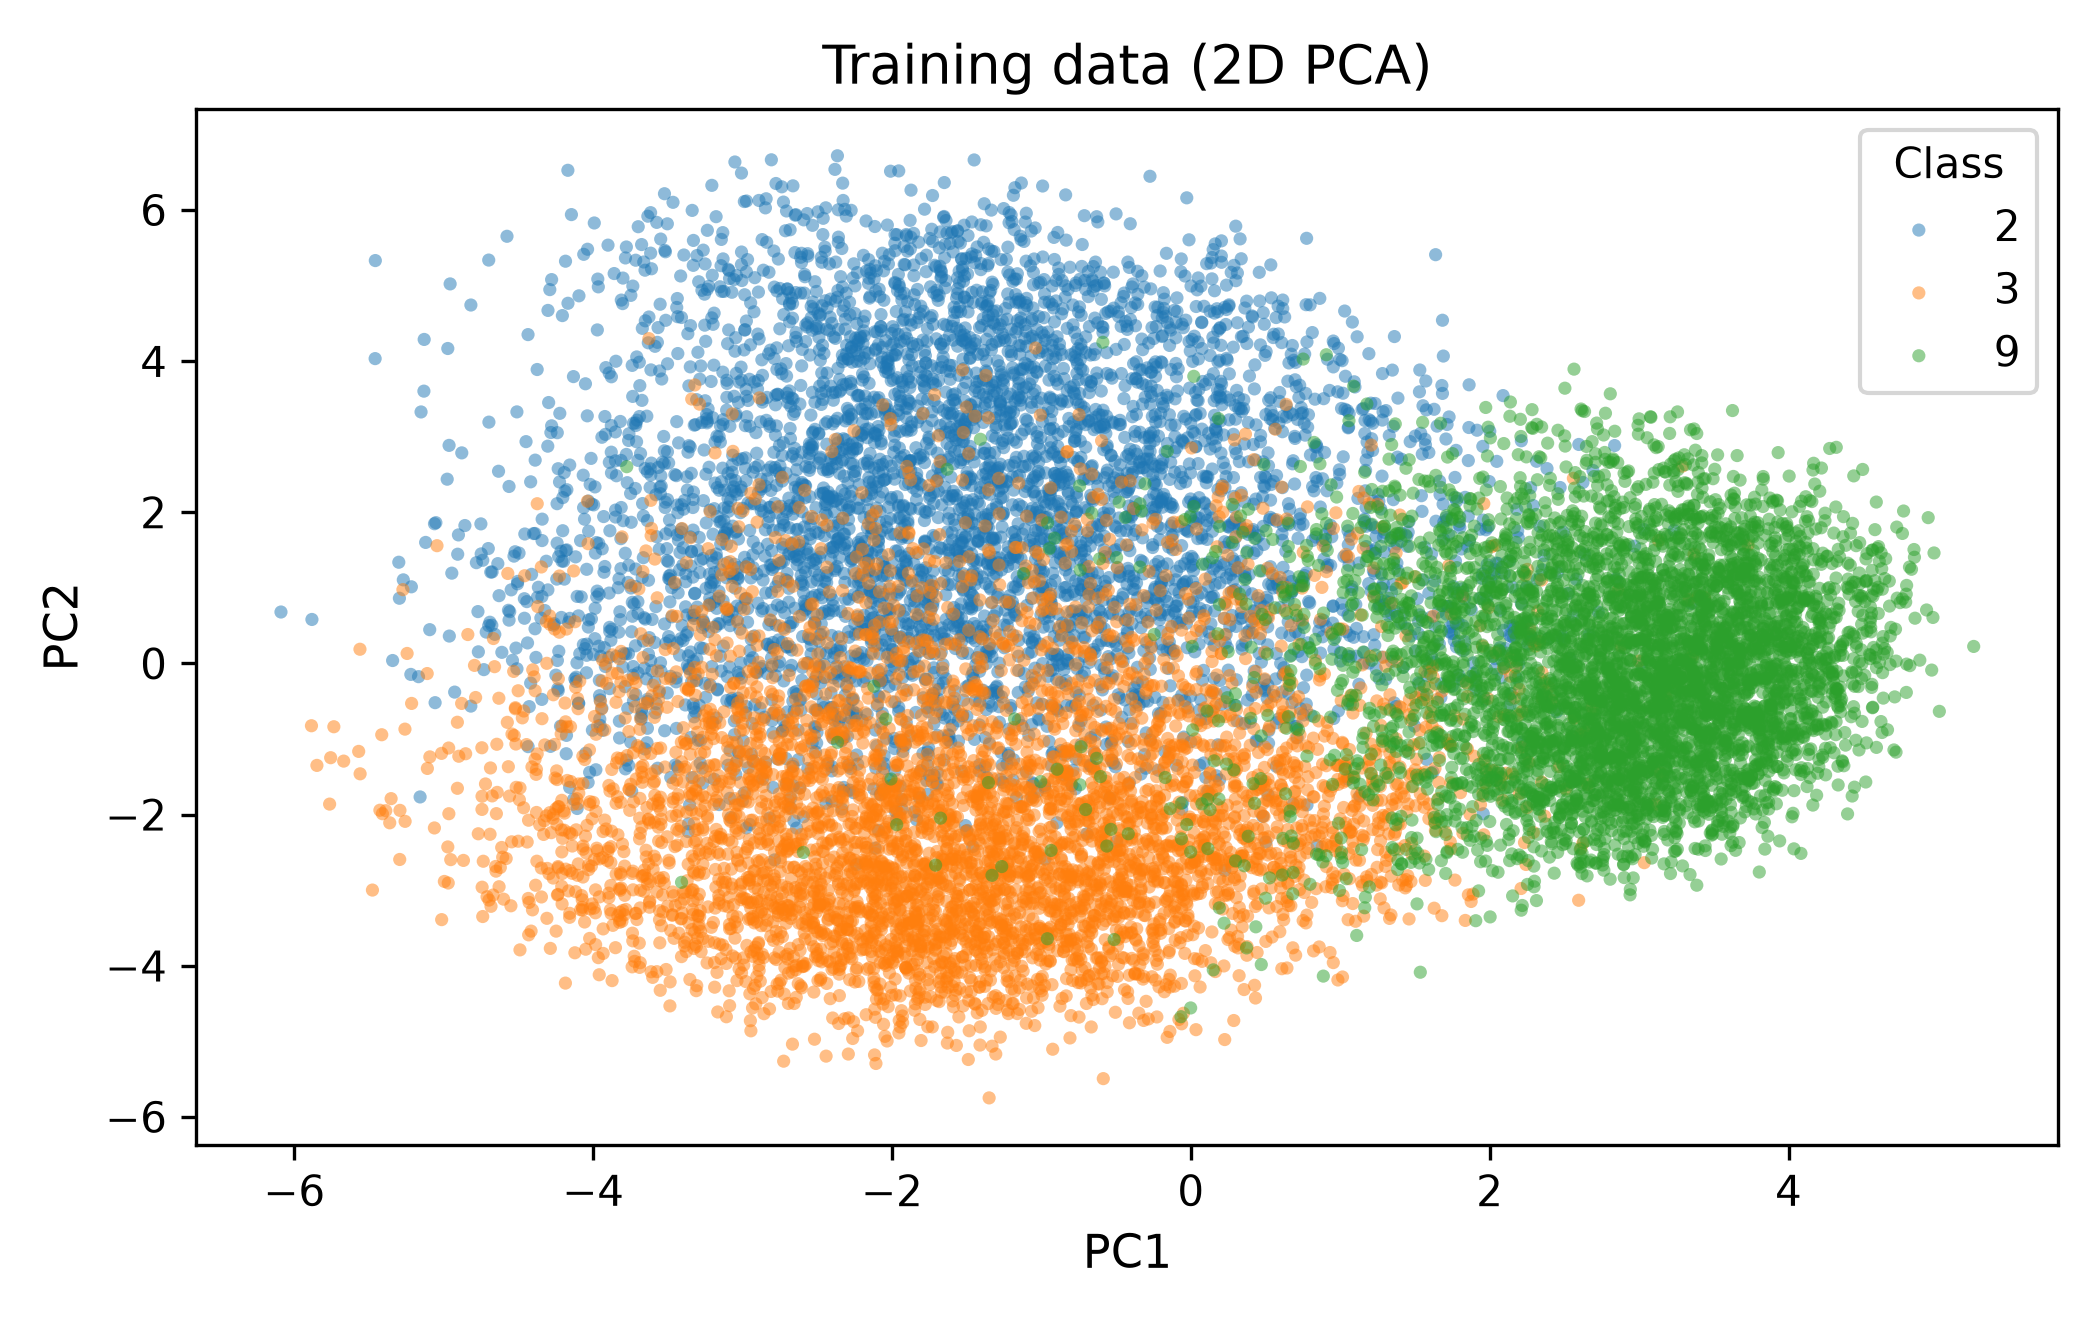
\includegraphics[width=0.90\linewidth]{mnist_pca.png}
\end{center}\end{minipage}\sectiongap
\noindent\begin{minipage}{\linewidth}
\textbf{Accuracy (\%)}\par
\begin{center}\small
\setlength{\tabcolsep}{9pt}
\renewcommand{\arraystretch}{1.15}
\begin{tabular}{lrrrr}\toprule
 & \multicolumn{2}{c}{Without PCA} & \multicolumn{2}{c}{With PCA} \\
\cmidrule(lr){2-3}\cmidrule(lr){4-5}
Classifier & Validation & Test & Validation & Test \\ \midrule
GMM & 96.65 & 97.31 & 98.12 & 98.66 \\
KNN & 98.59 & 98.92 & 98.84 & 99.08 \\
LDA & 94.27 & 95.31 & 93.86 & 95.67 \\
SVM & 99.11 & \textbf{99.34} & 99.25 & \textbf{99.48} \\
\bottomrule\end{tabular}\end{center}
\end{minipage}\par\clearpage
\noindent\begin{minipage}{\linewidth}
\begin{center}
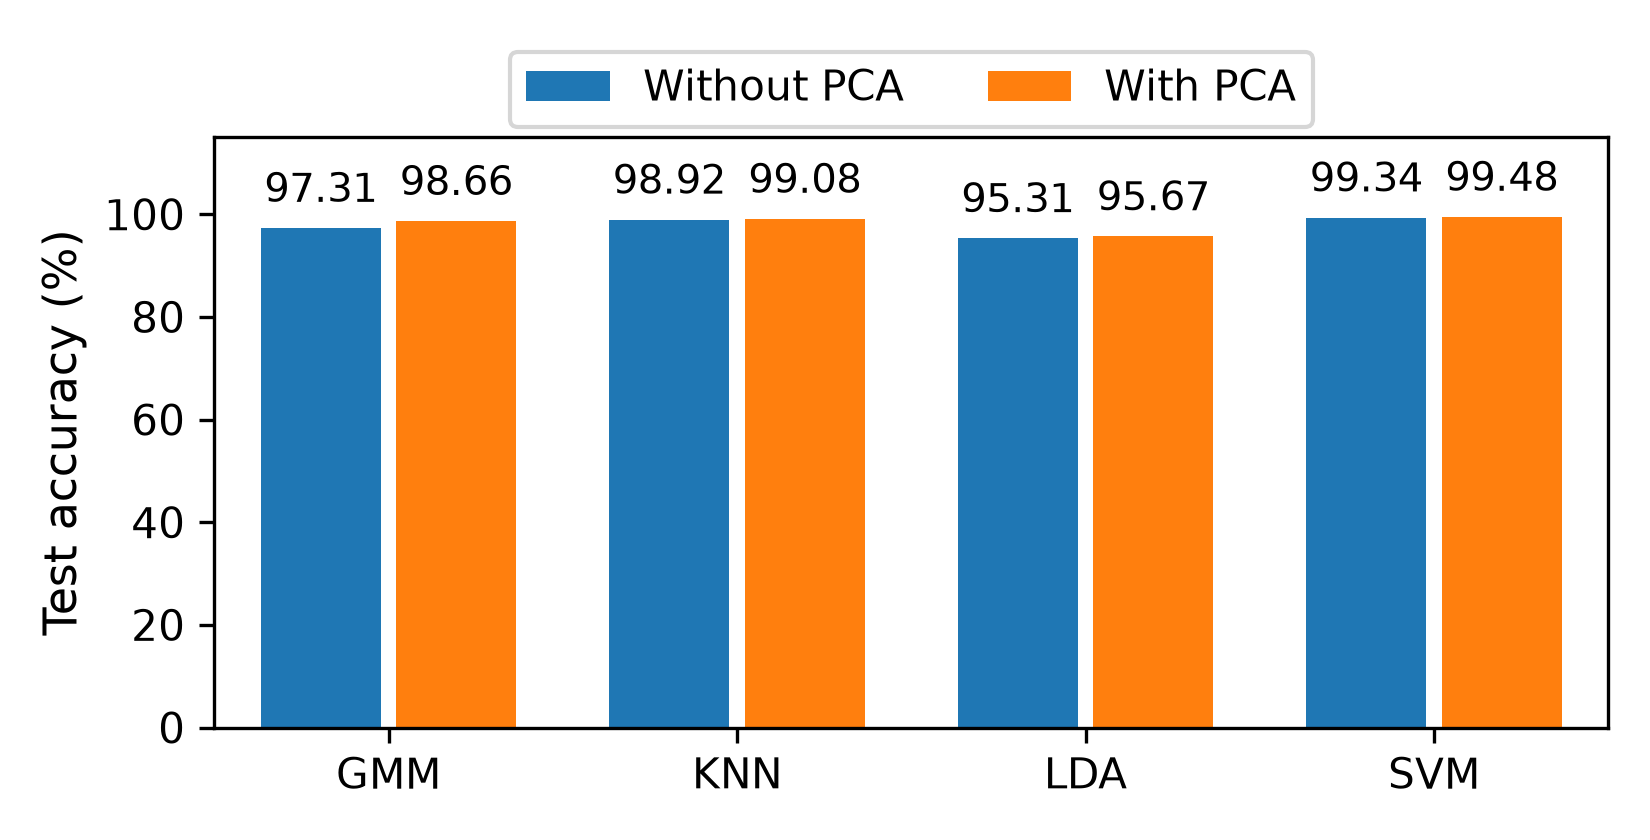
\includegraphics[width=0.70\linewidth]{mnist_accuracy.png}
\end{center}\end{minipage}\sectiongap
\noindent\begin{minipage}{\linewidth}
\textbf{Test confusion matrices}\hfill{\footnotesize Rows: actual; columns: predicted.}\par\smallskip
\textbf{Without PCA}\par\smallskip
\confusion{GMM}{rrr}{
 & \textbf{2} & \textbf{3} & \textbf{9} \\ \midrule
\textbf{2} & 1006 & 21 & 5 \\
\textbf{3} & 12 & 989 & 9 \\
\textbf{9} & 5 & 30 & 974 \\
}\hfill
\confusion{KNN}{rrr}{
 & \textbf{2} & \textbf{3} & \textbf{9} \\ \midrule
\textbf{2} & 1027 & 2 & 3 \\
\textbf{3} & 2 & 998 & 10 \\
\textbf{9} & 5 & 11 & 993 \\
}\hfill
\confusion{LDA}{rrr}{
 & \textbf{2} & \textbf{3} & \textbf{9} \\ \midrule
\textbf{2} & 987 & 24 & 21 \\
\textbf{3} & 32 & 955 & 23 \\
\textbf{9} & 12 & 31 & 966 \\
}\hfill
\confusion{SVM}{rrr}{
 & \textbf{2} & \textbf{3} & \textbf{9} \\ \midrule
\textbf{2} & 1029 & 1 & 2 \\
\textbf{3} & 3 & 1004 & 3 \\
\textbf{9} & 3 & 8 & 998 \\
}
\par\medskip
\textbf{With PCA}\par\smallskip
\confusion{GMM}{rrr}{
 & \textbf{2} & \textbf{3} & \textbf{9} \\ \midrule
\textbf{2} & 1022 & 5 & 5 \\
\textbf{3} & 4 & 998 & 8 \\
\textbf{9} & 5 & 14 & 990 \\
}\hfill
\confusion{KNN}{rrr}{
 & \textbf{2} & \textbf{3} & \textbf{9} \\ \midrule
\textbf{2} & 1027 & 1 & 4 \\
\textbf{3} & 2 & 998 & 10 \\
\textbf{9} & 1 & 10 & 998 \\
}\hfill
\confusion{LDA}{rrr}{
 & \textbf{2} & \textbf{3} & \textbf{9} \\ \midrule
\textbf{2} & 983 & 28 & 21 \\
\textbf{3} & 31 & 955 & 24 \\
\textbf{9} & 6 & 22 & 981 \\
}\hfill
\confusion{SVM}{rrr}{
 & \textbf{2} & \textbf{3} & \textbf{9} \\ \midrule
\textbf{2} & 1029 & 0 & 3 \\
\textbf{3} & 3 & 1004 & 3 \\
\textbf{9} & 0 & 7 & 1002 \\
}
\sectiongap
\textbf{Observations}\par

All of the four classifiers improved on the test after PCA to 50 dimensions, we believe that PCA has taken out some noise or unwanted variations along with it when it did the dimensionality reduction. SVM gets the best results on this split.

\end{minipage}\par\bigskip
\clearpage
\noindent\begin{minipage}{\linewidth}
{\Large\textbf{4. TIDIGITS}}\par\medskip
\begin{center}\small
\begin{tabular}{lrrrrrr}\toprule
Labels & Classes & Train & Validation & Test & Features $d$ & PCA $k$ \\ \midrule
$\{1,5,6\}$ & 3 & 810 & 270 & 270 & 4017 & 39 \\ \bottomrule
\end{tabular}\end{center}
\vspace{3mm}
\begin{center}
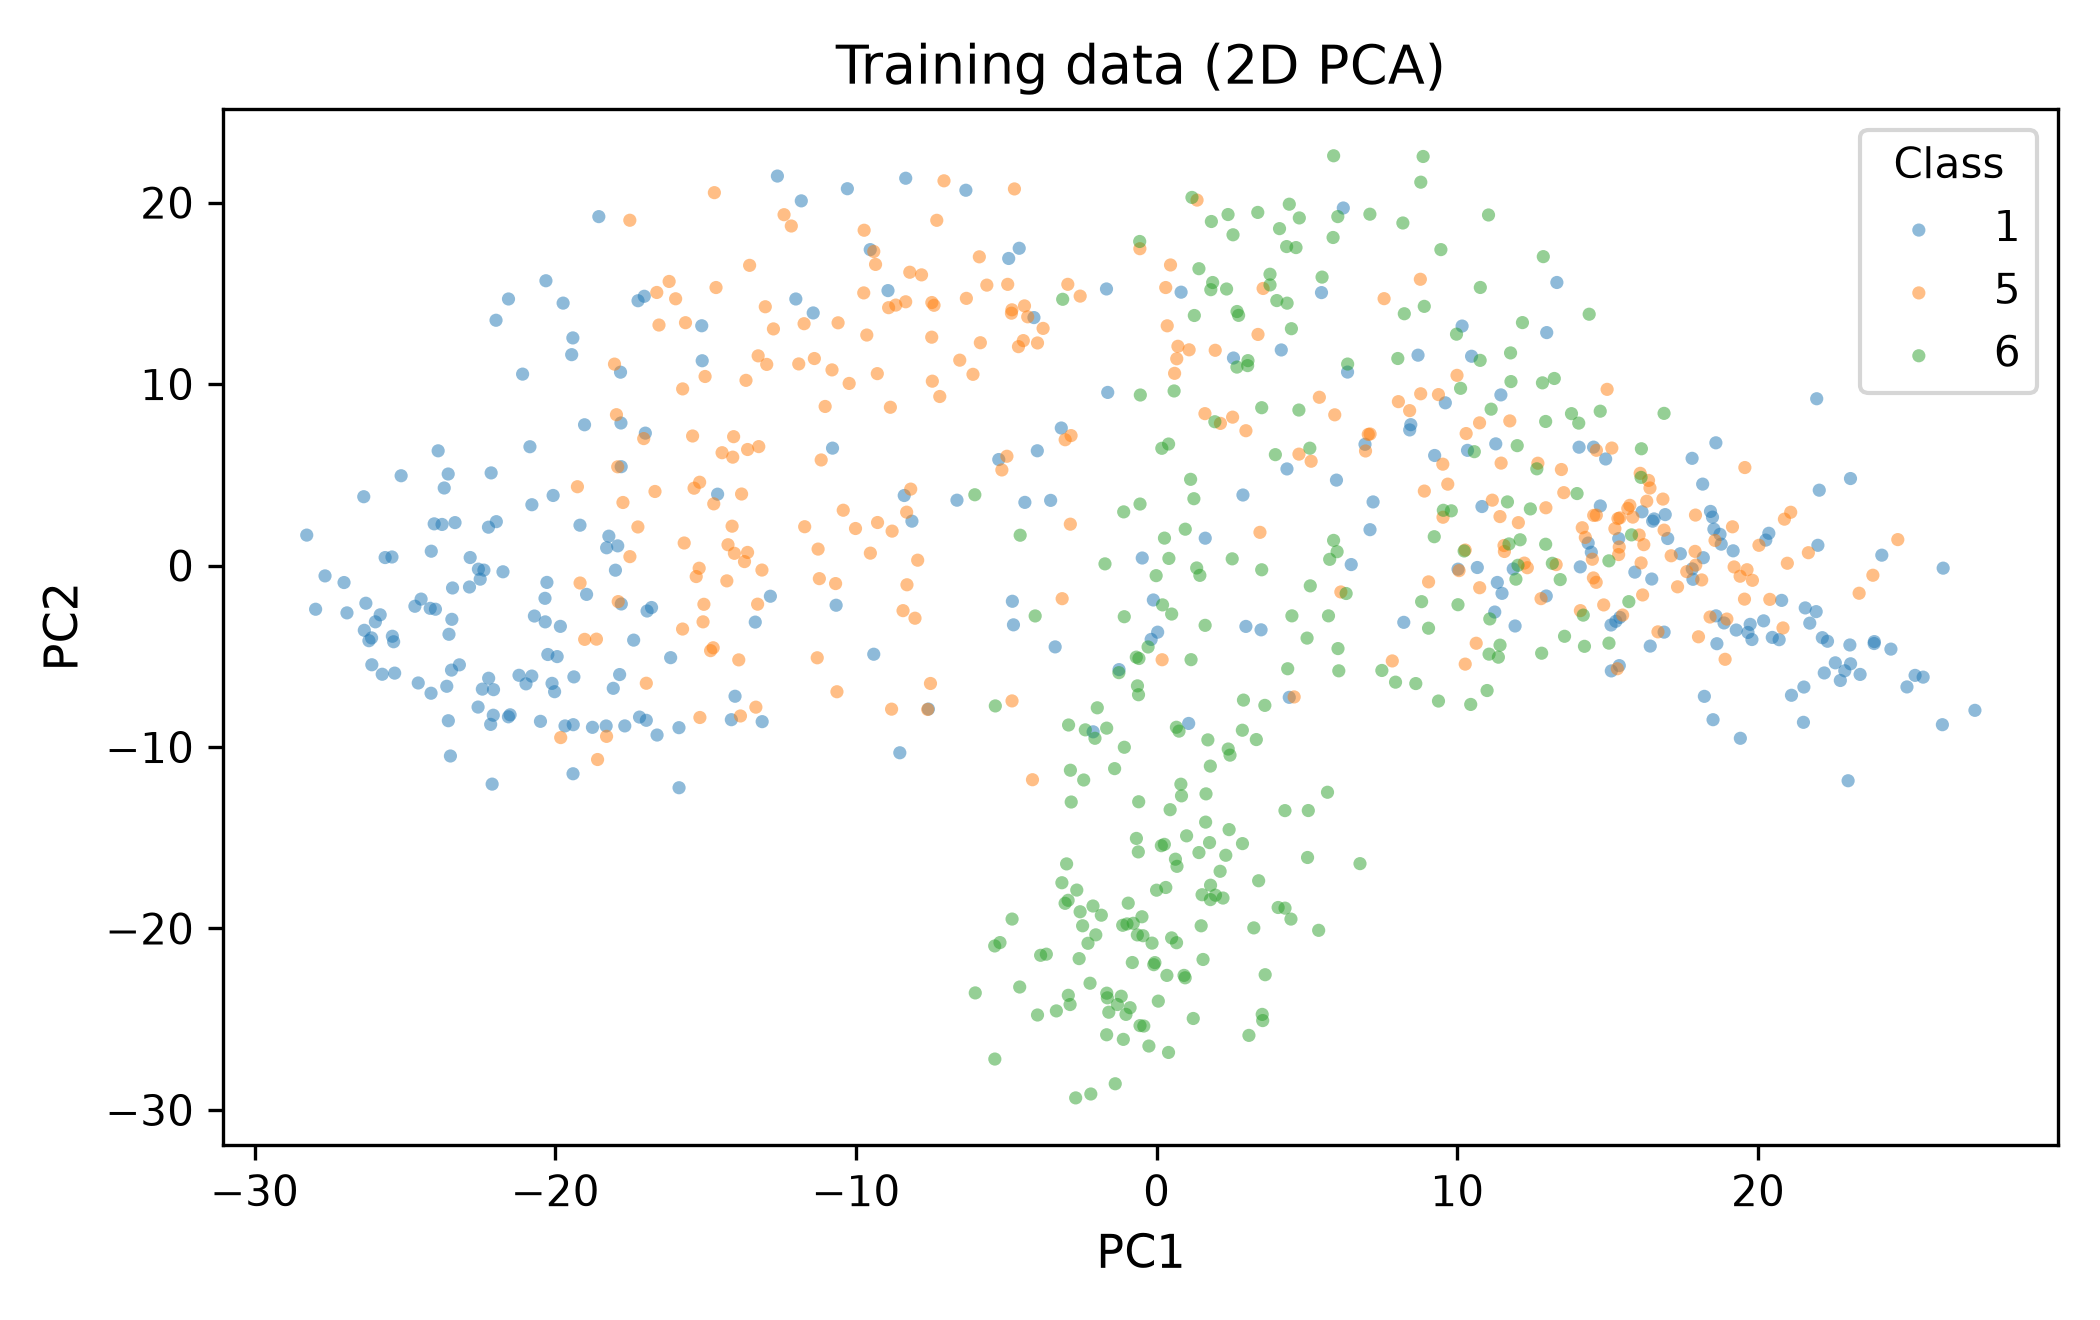
\includegraphics[width=0.90\linewidth]{tidigits_pca.png}
\end{center}\end{minipage}\sectiongap
\noindent\begin{minipage}{\linewidth}
\textbf{Accuracy (\%)}\par
\begin{center}\small
\setlength{\tabcolsep}{9pt}
\renewcommand{\arraystretch}{1.15}
\begin{tabular}{lrrrr}\toprule
 & \multicolumn{2}{c}{Without PCA} & \multicolumn{2}{c}{With PCA} \\
\cmidrule(lr){2-3}\cmidrule(lr){4-5}
Classifier & Validation & Test & Validation & Test \\ \midrule
GMM & 86.30 & 87.78 & 94.44 & 96.67 \\
KNN & 93.33 & \textbf{95.93} & 95.19 & \textbf{97.78} \\
LDA & 92.22 & 93.33 & 83.70 & 82.22 \\
SVM & 94.44 & 94.44 & 96.30 & \textbf{97.78} \\
\bottomrule\end{tabular}\end{center}
\end{minipage}\par\clearpage
\noindent\begin{minipage}{\linewidth}
\begin{center}
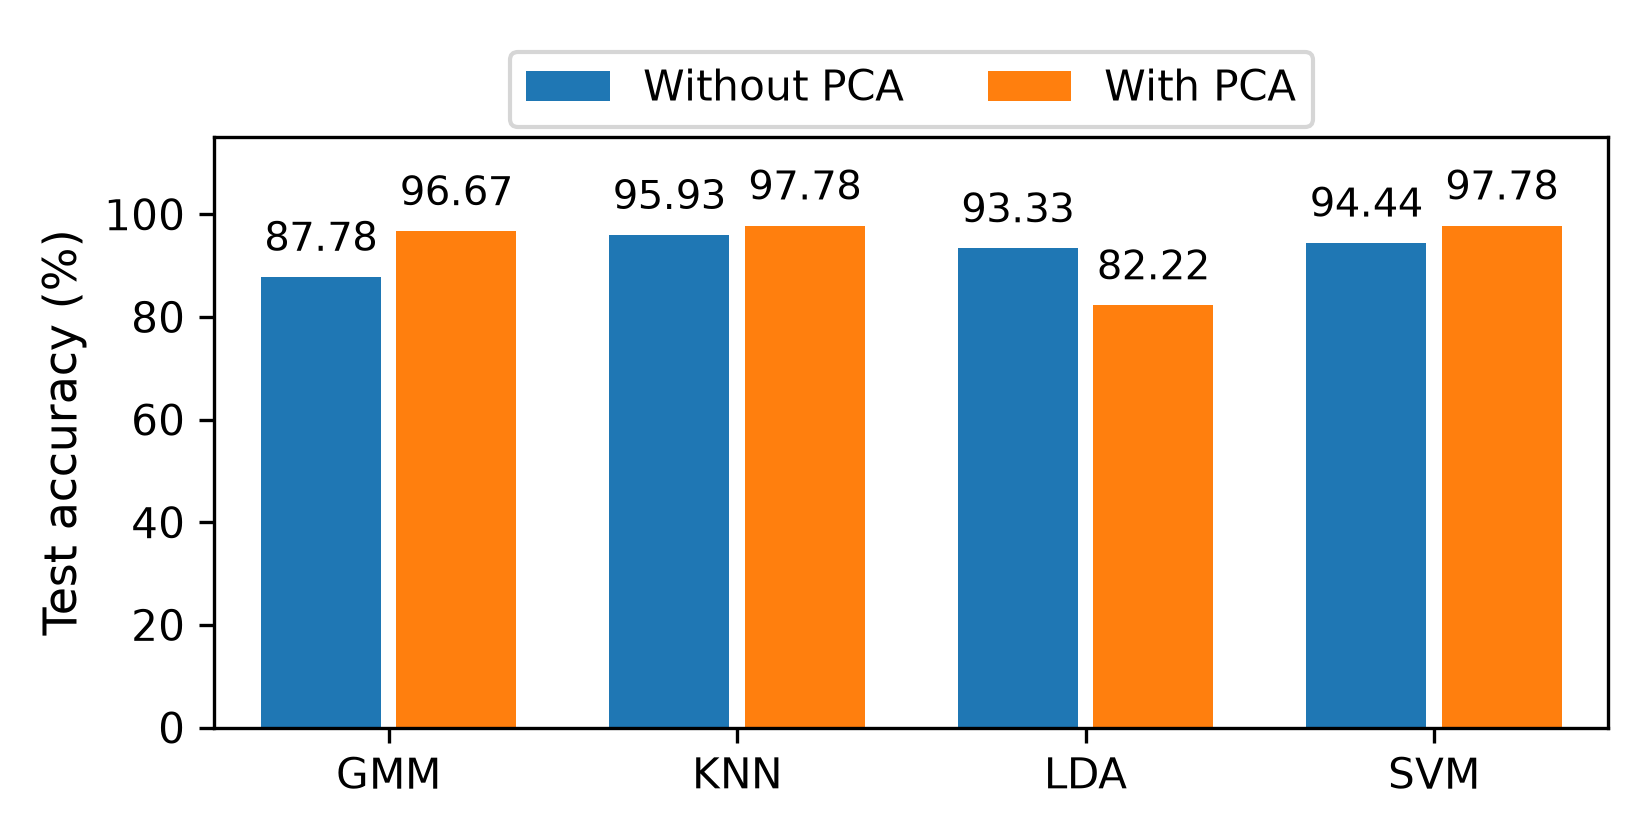
\includegraphics[width=0.70\linewidth]{tidigits_accuracy.png}
\end{center}\end{minipage}\sectiongap
\noindent\begin{minipage}{\linewidth}
\textbf{Test confusion matrices}\hfill{\footnotesize Rows: actual; columns: predicted.}\par\smallskip
\textbf{Without PCA}\par\smallskip
\confusion{GMM}{rrr}{
 & \textbf{1} & \textbf{5} & \textbf{6} \\ \midrule
\textbf{1} & 88 & 0 & 0 \\
\textbf{5} & 28 & 64 & 2 \\
\textbf{6} & 3 & 0 & 85 \\
}\hfill
\confusion{KNN}{rrr}{
 & \textbf{1} & \textbf{5} & \textbf{6} \\ \midrule
\textbf{1} & 88 & 0 & 0 \\
\textbf{5} & 6 & 88 & 0 \\
\textbf{6} & 5 & 0 & 83 \\
}\hfill
\confusion{LDA}{rrr}{
 & \textbf{1} & \textbf{5} & \textbf{6} \\ \midrule
\textbf{1} & 84 & 4 & 0 \\
\textbf{5} & 9 & 83 & 2 \\
\textbf{6} & 3 & 0 & 85 \\
}\hfill
\confusion{SVM}{rrr}{
 & \textbf{1} & \textbf{5} & \textbf{6} \\ \midrule
\textbf{1} & 82 & 1 & 5 \\
\textbf{5} & 3 & 86 & 5 \\
\textbf{6} & 0 & 1 & 87 \\
}
\par\medskip
\textbf{With PCA}\par\smallskip
\confusion{GMM}{rrr}{
 & \textbf{1} & \textbf{5} & \textbf{6} \\ \midrule
\textbf{1} & 85 & 3 & 0 \\
\textbf{5} & 4 & 89 & 1 \\
\textbf{6} & 0 & 1 & 87 \\
}\hfill
\confusion{KNN}{rrr}{
 & \textbf{1} & \textbf{5} & \textbf{6} \\ \midrule
\textbf{1} & 86 & 2 & 0 \\
\textbf{5} & 1 & 93 & 0 \\
\textbf{6} & 2 & 1 & 85 \\
}\hfill
\confusion{LDA}{rrr}{
 & \textbf{1} & \textbf{5} & \textbf{6} \\ \midrule
\textbf{1} & 73 & 15 & 0 \\
\textbf{5} & 17 & 69 & 8 \\
\textbf{6} & 7 & 1 & 80 \\
}\hfill
\confusion{SVM}{rrr}{
 & \textbf{1} & \textbf{5} & \textbf{6} \\ \midrule
\textbf{1} & 87 & 1 & 0 \\
\textbf{5} & 2 & 91 & 1 \\
\textbf{6} & 1 & 1 & 86 \\
}
\sectiongap
\textbf{Observations}\par

PCA down to 39 dimensions helps GMM, KNN and SVM test accuracy, but LDA drops from 93.33\% to 82.22\%. We think the answer to this lies in the fact that PCA retains the high-variance directions. But, that is not the necessarily the best direction for discrimination, May be LDA lost some of it's important directions that is useful to it's discrimination. KNN and SVM tie at 97.78\% after PCA.


\end{minipage}\par\bigskip
\end{document}
